% ----------------------------------------------------------------------------
%  3.3  Thực nghiệm trên dữ liệu chuẩn
% ----------------------------------------------------------------------------
\subsection{Tái hiện thí nghiệm trên dữ liệu Cosexp}\label{sec:cosexp}

Bộ dữ liệu Cosexp của hộp công cụ SVM-KM~\cite{canu2005} được bài báo gốc dùng để minh họa ảnh hưởng của số đặc trưng $M$. Các điểm được lấy đều trên miền $[0,5]\times[-1,1]$ và được gán nhãn theo dấu của $\cos\bigl(0{,}5\,e^{0{,}7x(1)}\bigr)-x(2)$, nên biên thật dao động ngày càng nhanh khi $x(1)$ tăng. Ta dùng đúng thiết lập của~\cite{huang2013} ($500$ điểm huấn luyện, $500$ điểm kiểm tra, PWL-C-SVM với ánh xạ cộng tính, $M$ từ $2$ đến $40$), nhưng lặp lại mỗi cấu hình trên $10$ bộ dữ liệu sinh độc lập và chạy thêm ánh xạ HH để so sánh (\cref{fig:cosexp}).

\begin{figure}[t]
\centering
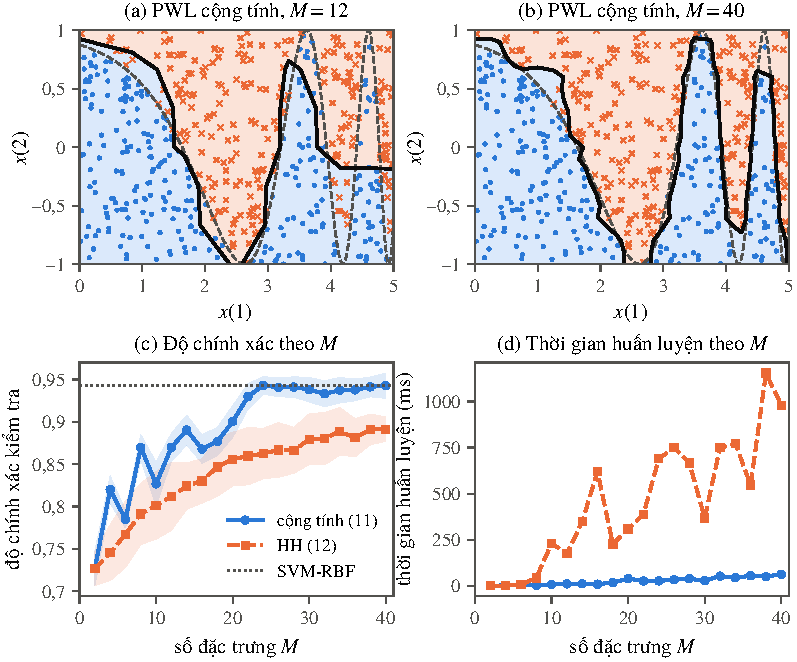
\includegraphics[width=0.78\linewidth]{fig_cosexp_M.pdf}
\caption[Tái hiện thí nghiệm Cosexp: ảnh hưởng của số đặc trưng]{Tái hiện thí nghiệm Cosexp (Hình~3 của~\cite{huang2013}), $10$ lần lặp. (a), (b) Biên của PWL-C-SVM cộng tính với $M=12$ và $M=40$ (nét liền) so với biên thật (nét đứt). (c) Độ chính xác trên tập kiểm tra theo $M$: đường là trung bình, dải màu là $\pm$ một độ lệch chuẩn; đường chấm là SVM hạt nhân Gauss. (d) Thời gian huấn luyện (trung vị) với $\gamma$ đã chọn.}
\label{fig:cosexp}
\end{figure}

Xu hướng mà bài báo gốc báo cáo được tái hiện đúng. Với $M=2$, bộ phân loại chỉ là tuyến tính và đạt $72{,}7\pm2{,}0\%$ (bài báo: $76{,}83\%$ với một lần chạy). Khi $M$ tăng, biên bám sát đường cong thật hơn; độ chính xác đạt $90{,}0\%$ tại $M=20=10n$ và ổn định quanh $94\%$ từ $M=24$, ngang SVM hạt nhân Gauss ($94{,}2\pm0{,}9\%$), trong khi thời gian huấn luyện vẫn dưới $0{,}1$ giây. Ánh xạ HH kém hẳn ($89{,}1\pm1{,}4\%$ tại $M=40$) dù về lý thuyết linh hoạt hơn, vì nhãn của Cosexp được xác định bởi một hàm cộng tính: ánh xạ cộng tính khớp đúng cấu trúc đó, còn các siêu phẳng ngẫu nhiên của HH phân tán khả năng biểu diễn vào những hướng không cần thiết. Cùng với \cref{sec:exp2d}, điều này cho một quy tắc thực hành, cũng là thứ tự mà bài báo gốc khuyến nghị~\cite[Mục~4]{huang2013}: thử ánh xạ cộng tính trước, vì nó rẻ, dễ diễn giải và đủ tốt khi tương tác giữa các biến yếu; chỉ chuyển sang HH khi có dấu hiệu tương tác mạnh.

% ----------------------------------------------------------------------------
\subsection{Mười bộ dữ liệu chuẩn}\label{sec:bench10}

\paragraph{Dữ liệu và giao thức.} Đề án dùng mười bộ dữ liệu phân loại nhị phân (\cref{tab:datasets}): bảy bộ có trong Bảng~1 của bài báo gốc và ba bộ (Banknote, Spambase, Sonar) được thêm vào để đa dạng hóa kích thước và số chiều. Mỗi bộ được chia ngẫu nhiên có phân tầng thành hai nửa huấn luyện và kiểm tra, lặp lại $10$ lần ($5$ lần với Spambase, do chi phí tinh chỉnh các mô hình hạt nhân); với Magic, tập huấn luyện gồm $2.000$ điểm như trong bài báo gốc. Tham số được chọn bằng kiểm định chéo $10$ phần trên tập huấn luyện: $\gamma\in\{2^{-5},2^{-3},\dots,2^{11}\}$ cho mọi mô hình SVM, $1/\sigma^2\in\{2^{-15},2^{-13},\dots,2^{3}\}$ cho hạt nhân Gauss theo khuyến nghị của~\cite{hsu2003}, và hệ số phạt $L_2$ trong $\{10^{-4},10^{-3},\dots,1\}$ cho mạng nơ-ron. Chín phương pháp được so sánh: SVM tuyến tính; SVM và LS-SVM hạt nhân Gauss; kNN với $k=1$ như trong bài báo; Ik-SVM; mạng nơ-ron một lớp ẩn gồm $9n$ nơ-ron ReLU --- bằng số đặc trưng bản lề của PWL-SVM dạng HH --- huấn luyện bằng L-BFGS~\cite{liu1989}; và ba biến thể PWL-SVM với $M/n=10$ theo đúng quy tắc của bài báo: PWL-C-SVM và PWL-LS-SVM với ánh xạ cộng tính lưới đều, và PWL-C-SVM với ánh xạ HH chuẩn hóa $|p(1)|=1$.

\begin{table}[t]
\centering
\caption[Mười bộ dữ liệu chuẩn]{Mười bộ dữ liệu chuẩn, sắp theo số chiều $n$ (sau khi bỏ các cột hằng). $N$ là số mẫu, cột cuối là số mẫu huấn luyện/kiểm tra trong mỗi lần chia.}
\label{tab:datasets}
\small
\renewcommand{\arraystretch}{1.15}
\setlength{\tabcolsep}{4.5pt}
\begin{tabular}{@{}l l r r r r@{}}
\toprule
\textbf{Tên} & \textbf{Nội dung} & $N$ & $n$ & \begin{tabular}[b]{@{}c@{}}\textbf{\% lớp}\\ \textbf{$+1$}\end{tabular} & \begin{tabular}[b]{@{}c@{}}\textbf{Huấn luyện/}\\ \textbf{kiểm tra}\end{tabular}\\
\midrule
Haberman & sống sót sau phẫu thuật ung thư vú & 306 & 3 & 26{,}5 & 153/153\\
Transfusion & hiến máu tình nguyện & 748 & 4 & 23{,}8 & 374/374\\
Banknote & xác thực tiền giấy & 1.372 & 4 & 44{,}5 & 686/686\\
Pima & bệnh tiểu đường & 768 & 8 & 34{,}9 & 384/384\\
Breast & ung thư vú Wisconsin (bản gốc) & 699 & 9 & 34{,}5 & 349/350\\
Magic & kính thiên văn tia gamma & 19.020 & 10 & 35{,}2 & 2.000/17.020\\
Parkinsons & bệnh Parkinson (giọng nói) & 195 & 22 & 75{,}4 & 97/98\\
Ionosphere & tín hiệu radar tầng điện li & 351 & 33 & 64{,}1 & 175/176\\
Spambase & thư rác & 4.601 & 57 & 39{,}4 & 2.300/2.301\\
Sonar & tín hiệu sonar (đá hay mìn) & 208 & 60 & 53{,}4 & 104/104\\
\bottomrule
\end{tabular}
\end{table}


\begin{table}[t]
\centering
\caption[Độ chính xác trên mười bộ dữ liệu chuẩn]{Độ chính xác trung bình trên tập kiểm tra (\%) qua $10$ lần chia ngẫu nhiên ($5$ lần với Spambase). In đậm: giá trị cao nhất mỗi hàng. Dòng cuối là hạng trung bình trên mười bộ dữ liệu ($1$ là tốt nhất). Độ lệch chuẩn được cho ở \cref{tab:appendix-bench} (Phụ lục~B).}
\label{tab:bench}
\footnotesize
\setlength{\tabcolsep}{3pt}
\renewcommand{\arraystretch}{1.18}
\resizebox{\linewidth}{!}{%
\begin{tabular}{@{}l r r r r r r r r r@{}}
\toprule
\textbf{Dữ liệu} & \begin{tabular}[b]{@{}c@{}}SVM\\tuyến tính\end{tabular} & \begin{tabular}[b]{@{}c@{}}SVM-\\RBF\end{tabular} & \begin{tabular}[b]{@{}c@{}}LS-SVM-\\RBF\end{tabular} & \begin{tabular}[b]{@{}c@{}}kNN\\$(k=1)$\end{tabular} & \begin{tabular}[b]{@{}c@{}}Ik-\\SVM\end{tabular} & \begin{tabular}[b]{@{}c@{}}MLP-\\ReLU\end{tabular} & \begin{tabular}[b]{@{}c@{}}PWL-C\\cộng tính\end{tabular} & \begin{tabular}[b]{@{}c@{}}PWL-LS\\cộng tính\end{tabular} & \begin{tabular}[b]{@{}c@{}}PWL-C\\HH\end{tabular}\\
\midrule
Haberman & 72{,}5 & 73{,}3 & 73{,}4 & 65{,}7 & 72{,}0 & 72{,}4 & 73{,}2 & 72{,}6 & \textbf{73{,}5}\\
Transfusion & 76{,}5 & 77{,}6 & 77{,}7 & 68{,}4 & 76{,}7 & \textbf{78{,}6} & 76{,}3 & 77{,}4 & 76{,}3\\
Banknote & 98{,}6 & \textbf{100{,}0} & \textbf{100{,}0} & 99{,}8 & 99{,}9 & 99{,}9 & 99{,}9 & 99{,}5 & 99{,}9\\
Pima & \textbf{76{,}7} & 76{,}1 & 76{,}6 & 70{,}8 & 76{,}0 & \textbf{76{,}7} & 76{,}3 & 76{,}5 & 76{,}2\\
Breast & 96{,}6 & 96{,}5 & 96{,}4 & 95{,}3 & 96{,}4 & \textbf{96{,}8} & 96{,}3 & 96{,}0 & 95{,}6\\
Magic & 79{,}0 & 85{,}5 & 85{,}6 & 78{,}3 & 85{,}0 & \textbf{85{,}7} & 84{,}8 & 84{,}4 & 84{,}3\\
Parkinsons & 85{,}4 & 89{,}9 & 91{,}4 & \textbf{93{,}7} & 89{,}4 & 90{,}6 & 86{,}2 & 89{,}3 & 85{,}5\\
Ionosphere & 86{,}2 & 93{,}4 & \textbf{93{,}8} & 86{,}4 & 91{,}1 & 88{,}0 & 89{,}7 & 87{,}7 & 87{,}0\\
Spambase & 93{,}0 & 93{,}6 & 93{,}4 & 88{,}8 & \textbf{94{,}6} & 93{,}9 & 93{,}4 & 92{,}6 & 82{,}1\\
Sonar & 75{,}2 & 84{,}3 & \textbf{84{,}5} & 81{,}2 & 82{,}0 & 81{,}9 & 80{,}2 & 79{,}8 & 76{,}2\\
\midrule
Hạng trung bình & 6{,}55 & 3{,}15 & 2{,}35 & 7{,}40 & 4{,}60 & 3{,}00 & 5{,}35 & 6{,}00 & 6{,}60\\
\bottomrule
\end{tabular}}
\end{table}


\begin{table}[t]
\centering
\caption[So sánh theo cặp với PWL-C-SVM cộng tính]{So sánh theo cặp giữa PWL-C-SVM cộng tính và từng phương pháp khác trên mười bộ dữ liệu: số bộ mà PWL-C-SVM cao hơn / bằng / thấp hơn và chênh lệch trung bình (tính trên các giá trị của \cref{tab:bench}), cùng giá trị $p$ của kiểm định dấu hạng Wilcoxon hai phía trên độ chính xác trung bình chưa làm tròn, chưa hiệu chỉnh cho so sánh bội.}
\label{tab:wilcoxon}
\small
\renewcommand{\arraystretch}{1.18}
\begin{tabular}{@{}l c r r@{}}
\toprule
\textbf{Phương pháp so sánh} & \textbf{Cao hơn / bằng / thấp hơn} & \textbf{Chênh lệch TB} & $p$\\
\midrule
SVM tuyến tính & 7 / 0 / 3 & $+1{,}66$ & 0{,}037\\
SVM-RBF & 1 / 0 / 9 & $-1{,}39$ & 0{,}020\\
LS-SVM-RBF & 0 / 1 / 9 & $-1{,}65$ & 0{,}002\\
kNN ($k=1$) & 8 / 0 / 2 & $+2{,}79$ & 0{,}084\\
Ik-SVM & 2 / 1 / 7 & $-0{,}68$ & 0{,}105\\
MLP-ReLU & 2 / 1 / 7 & $-0{,}82$ & 0{,}139\\
PWL-LS-SVM cộng tính & 7 / 0 / 3 & $+0{,}05$ & 0{,}432\\
PWL-C-SVM HH & 7 / 2 / 1 & $+1{,}97$ & 0{,}027\\
\bottomrule
\end{tabular}
\end{table}


\paragraph{Kết quả.} Ba phương pháp dẫn đầu về độ chính xác (\cref{tab:bench}) là LS-SVM hạt nhân Gauss, mạng nơ-ron và SVM hạt nhân Gauss, với hạng trung bình lần lượt $2{,}35$, $3{,}00$ và $3{,}15$; PWL-C-SVM cộng tính đứng giữa bảng (hạng $5{,}35$), trên SVM tuyến tính ($6{,}55$) và kNN ($7{,}40$). Trên năm bộ Haberman, Transfusion, Banknote, Pima và Breast, mọi phương pháp dựa trên SVM, kể cả SVM tuyến tính, chênh nhau không quá khoảng $1{,}5$ điểm phần trăm: một biên tuyến tính đã gần như đủ tốt. Trên bốn bộ Magic, Parkinsons, Ionosphere và Sonar, nơi SVM tuyến tính kém SVM hạt nhân Gauss từ $4$ đến $9$ điểm, PWL-C-SVM cộng tính thu hẹp đáng kể khoảng cách trên ba bộ (hơn SVM tuyến tính $5{,}8$ điểm trên Magic, $3{,}5$ điểm trên Ionosphere và $5{,}0$ điểm trên Sonar) nhưng vẫn kém SVM hạt nhân Gauss từ $0{,}7$ đến $4{,}1$ điểm. Để so sánh hai bộ phân loại trên nhiều bộ dữ liệu, Demšar~\cite{demsar2006} khuyến nghị kiểm định dấu hạng Wilcoxon; \cref{tab:wilcoxon} áp dụng kiểm định này cho PWL-C-SVM cộng tính và từng phương pháp khác. Với hai so sánh chính của câu hỏi CH1, PWL-C-SVM cộng tính kém SVM hạt nhân Gauss ($p=0{,}020$) và cao hơn SVM tuyến tính trên bảy trong mười bộ, với chênh lệch trung bình $1{,}7$ điểm ($p=0{,}037$); sau hiệu chỉnh Holm cho hai phép so sánh, cả hai khác biệt vẫn có ý nghĩa ở mức $5\%$ (giá trị $p$ hiệu chỉnh đều bằng $0{,}039$). Các giá trị $p$ khác trong \cref{tab:wilcoxon} chưa được hiệu chỉnh cho so sánh bội: nếu hiệu chỉnh Holm cho cả tám phép so sánh, chỉ khác biệt so với LS-SVM hạt nhân Gauss còn có ý nghĩa ở mức $5\%$. Với chỉ mười bộ dữ liệu, các kiểm định này có lực thấp, nên “không bác bỏ” không có nghĩa là “tương đương”.

\paragraph{So với bài báo gốc.} Kết quả trên không xác nhận nhận định của bài báo gốc rằng PWL-SVM có độ chính xác tương đương SVM hạt nhân Gauss~\cite{huang2013}. Nguyên nhân chính là bài báo chỉ dùng một lần chia dữ liệu: trên các bộ nhỏ như Parkinsons ($98$ điểm kiểm tra), độ lệch chuẩn giữa các lần chia lên tới $2$--$4$ điểm phần trăm, và bài báo báo cáo độ chính xác $100\%$ cho PWL-C-SVM trên bộ này, trong khi trung bình qua mười lần chia chỉ là $86{,}2\%$. Ngược lại, lợi thế về kích thước mô hình được xác nhận rõ ràng: với ánh xạ cộng tính, PWL-C-SVM cần từ $64$ đến $1.261$ số thực, nhỏ hơn SVM hạt nhân Gauss từ $2{,}5$ đến $36$ lần (Phụ lục~B). Trường hợp đáng chú ý nhất là Magic: PWL-C-SVM đạt $84{,}8\%$ so với $85{,}5\%$ của SVM hạt nhân Gauss với một mô hình gồm $211$ số thực thay vì $7.694$.

\paragraph{Ánh xạ HH.} PWL-C-SVM với ánh xạ HH có hạng trung bình thấp ($6{,}60$), chủ yếu do quy tắc sinh tham số chứ không phải do mô hình. Trên Spambase, ở lần chia đầu tiên, mô hình thất bại hoàn toàn ($40{,}0\%$, thấp hơn cả tỉ lệ $60{,}6\%$ của lớp đa số), trong khi ở bốn lần chia còn lại nó đạt từ $91{,}0\%$ đến $93{,}7\%$. Nguyên nhân là dữ liệu này rất thưa (gần $78\%$ giá trị bằng $0$ sau khi chuẩn hóa), nên nhiều siêu phẳng đi qua các điểm lấy đều trong hình hộp $[0,1]^{57}$ không cắt qua vùng dữ liệu, còn quy tắc $|p(1)|=1$ (\cref{rem:scale}) làm giá trị lớn nhất của các đặc trưng trên tập huấn luyện dao động từ $423$ đến $3{,}3\cdot10^{5}$ giữa các lần chia, khiến bài toán tối ưu bị điều kiện hóa rất kém. Chỉ cần chuẩn hóa $\|p\|_2=1$, PWL-C-SVM HH đạt $93{,}4\pm0{,}2\%$ trên Spambase. Ngoài ra, mạng nơ-ron với cùng số nơ-ron ẩn tốt hơn PWL-C-SVM HH trên tám trong mười bộ: học lớp ẩn từ dữ liệu có lợi hơn nhiều so với sinh nó ngẫu nhiên, và đó là cái giá của tính lồi đã nêu ở Mục~\ref{sec:pwlsvm}.

% ----------------------------------------------------------------------------
\subsection{Ảnh hưởng của số đặc trưng và của quy tắc chọn tham số}\label{sec:sensitivity}

Để trả lời câu hỏi CH3 một cách có kiểm soát, ta cố định mô hình là PWL-LS-SVM, giải chính xác bằng hồi quy ridge (\cref{prop:ridge}) để loại trừ ảnh hưởng của bộ giải, và thay đổi hai yếu tố: số đặc trưng trên mỗi chiều $M/n\in\{1,2,3,5,10,20\}$ và quy tắc chọn tham số --- ánh xạ cộng tính với lưới đều (quy tắc của bài báo gốc) hoặc lưới phân vị (\cref{rem:quantile}), ánh xạ HH với $|p(1)|=1$ (quy tắc của bài báo gốc) hoặc $\|p\|_2=1$ (\cref{rem:scale}). Thí nghiệm dùng ba bộ dữ liệu có đặc điểm khác nhau --- Ionosphere ($n=33$), Magic ($n=10$, nhiều dữ liệu) và Spambase ($n=57$, rất thưa) --- với $5$ lần chia như ở Mục~\ref{sec:bench10} và $\gamma$ chọn bằng kiểm định chéo $5$ phần (\cref{fig:sensitivity}).

\begin{figure}[t]
\centering
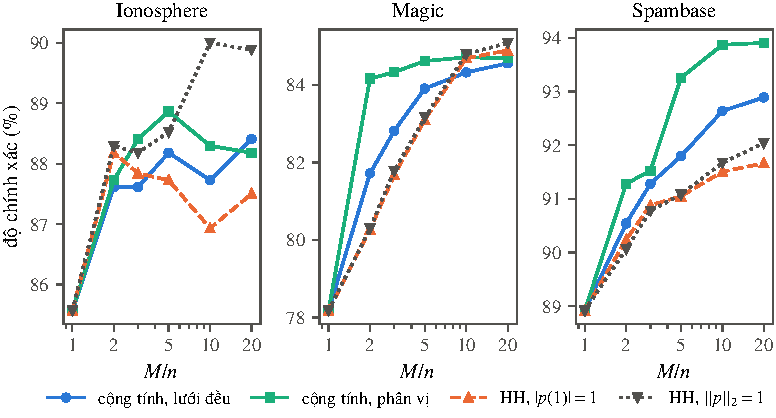
\includegraphics[width=0.84\linewidth]{fig_sensitivity.pdf}
\caption[Ảnh hưởng của số đặc trưng và quy tắc chọn tham số]{Độ chính xác trung bình (qua $5$ lần chia) của PWL-LS-SVM theo số đặc trưng trên mỗi chiều $M/n$, với bốn quy tắc chọn tham số. $M/n=1$ ứng với bộ phân loại tuyến tính.}
\label{fig:sensitivity}
\end{figure}

Có ba nhận xét. Thứ nhất, độ chính xác tăng nhanh khi $M/n$ tăng từ $1$ và bão hòa quanh $M/n=5$--$10$, phù hợp với quy tắc $M=10n$ của bài báo gốc. Thứ hai, lưới phân vị tốt hơn hoặc ngang lưới đều trên cả ba bộ, rõ nhất khi phân bố lệch: trên Magic, nó đạt $84{,}2\%$ ngay với $M/n=2$, trong khi lưới đều cần $M/n=10$ để đạt $84{,}3\%$; trên Spambase, nó đạt $93{,}9\%$ so với $92{,}6\%$ của lưới đều ở $M/n=10$ mà chỉ dùng $156$ thay vì $570$ đặc trưng, vì các nút trùng nhau bị loại bỏ. Thứ ba, ánh xạ HH cần nhiều đặc trưng hơn hẳn mới đuổi kịp ánh xạ cộng tính: trên Magic, nó chỉ ngang lưới phân vị khi $M/n\ge10$ (nhỉnh hơn $0{,}4$ điểm ở $M/n=20$), trên Spambase nó kém ở mọi giá trị của $M/n$; chỉ trên Ionosphere, nơi tương tác giữa các biến có vai trò, HH với $\|p\|_2=1$ tốt nhất rõ rệt ($90{,}0\%$ ở $M/n=10$, so với $86{,}9\%$ với $|p(1)|=1$). Chuẩn hóa $\|p\|_2=1$ không làm kết quả xấu đi đáng kể ở bất kỳ cấu hình nào. Từ đó rút ra quy trình được dùng cho dữ liệu dạng bảng ở phần còn lại của chương: ánh xạ cộng tính, nút theo phân vị, $M/n$ từ $5$ đến $10$; chỉ dùng ánh xạ HH, với các siêu phẳng được chuẩn hóa, khi có dấu hiệu tương tác mạnh giữa các biến.

